\subsection{Đề 3}
\Opensolutionfile{ans}[ans/ans-1-OTHK1-De3-LC]
\caulc
\begin{ex}%[1D1H5-3]
Tổng $T$ các nghiệm của phương trình $\sin x=\dfrac{1}{2}$ trên $(0;3\pi)$ bằng
	\choice
{$T=3\pi$}
{$T=\pi$}
{$T=5\pi$}
{\True $T=6\pi$}
	\loigiai{
	Ta có $\sin x=\dfrac{1}{2}=\sin \dfrac{\pi}{6}\Leftrightarrow \hoac{&x=\dfrac{\pi}{6}+k2\pi\\&x=\dfrac{5\pi}{6}+k2\pi}$.\\
	Do $x\in (0;3\pi)$ nên các nghiệm của phương trình là $x=\dfrac{\pi}{6}$, $x=\dfrac{13\pi}{6}$, $x=\dfrac{5\pi}{6}$, $x=\dfrac{17\pi}{6}$. Suy ra tổng các nghiệm là $T=6\pi$.
	}
\end{ex}
\begin{ex}%[1D2H3-2]
	Người ta trồng $2047$ cây theo hình tam giác như sau: hàng thứ nhất có $1$ cây, hàng thứ hai có $2$ cây, hàng thứ ba có $4$ cây,\ldots , hàng thứ $n$ có $2^{n-1}$ cây. Người ta có thể trồng bao nhiêu hàng cây với cách trồng này?
	\choice
	{\True $11$ hàng} 
	{$12$ hàng}
	{$10$ hàng} 
	{$15$ hàng}
	\loigiai
	{
		Theo đề bài ta có
		\begin{eqnarray*}
			&&1+2+4+\ldots +2^{n-1}=2047\\
			&\Leftrightarrow &2^{n}-1=2047\\
			&\Leftrightarrow &n=11.
		\end{eqnarray*}
		Vậy người ta có thể trồng $11$ hàng cây với cách trồng này.
	}
\end{ex}
\begin{ex}%[1D3N1-2]
	Tính 	$L=\displaystyle \lim \dfrac{n-1}{n^3 +3}$ 
	\choice{$ L=2 $}
	{$L=3 $}
	{$L= 1 $}
	{\True $L= 0 $}
	\loigiai{$L=\displaystyle \lim \dfrac{n-1}{n^3 +3}=\displaystyle \lim \dfrac{\dfrac{1}{n^2}-\dfrac{1}{n^3}}{1 +\dfrac{1}{n^3}}=\dfrac{0}{1}=0.$
	}
\end{ex}
\begin{ex}%[1D3H3-3] %[Dự án đề kiểm tra Toán 11 GHKI NH23-24- Nguyễn Sơn]%[THPT NGUYỄN CHÍ THANH - Tp HCM]
	Giá trị $ a $ để hàm số $ f(x)=\heva{&\dfrac{3x^2+x-4}{x-1}&, \text{khi}x\ne1 \\& a+2 & ,\text{khi} x=1} $ liên tục tại $ x_0 =1$ là
	\choice{$a=1$}{\True $a=5$}{$a=2$}{$a=-2$}
	\loigiai
	{
		\begin{itemize}
		\item $ f(1)=a+2 $.
		\item $ \lim\limits_{x \to 1} f(x)=\lim\limits_{x\to 1} \dfrac{3x^2+x-4}{x-1} =\lim\limits_{x \to 1}\dfrac{(x-1)(3x+4)}{x-1}=\lim\limits_{x\to 1}(3x+4)=7$.
	\end{itemize}
		Để hàm số liên tục tại $ x_0=1 $ thì $ \lim\limits_{x\to 1}f(x) =f(1)\Leftrightarrow 7=a+2 \Leftrightarrow a=5$.
		
	}
\end{ex}
\begin{ex}%[1D3N2-3]
	Giá trị của	$\lim\limits_{x\to -2}\dfrac{4x^3 -1}{3x^2 +x +2}$ có kết quả là
	\choice{\True $ -\dfrac{11}{4}$}
	{$-\infty $}
	{$\dfrac{11}{4} $}
	{ $ +\infty $}
	\loigiai{
		Ta có $\lim\limits_{x\to -2}\dfrac{4x^3 -1}{3x^2 +x +2}=\dfrac{4\cdot(-2)^3 -1}{3\cdot(-2)^2 +-2 +2}=\dfrac{-11}{4}$.}
\end{ex}
\begin{ex}%[1H4N4-1]
	Quan hệ song song trong không gian có tính chất nào trong các tính chất sau?
	\choice
	{\True Nếu hai mặt phẳng $(P)$ và $(Q)$ song song với nhau thì mọi đường thẳng nằm trong $(P)$ đều song song với $(Q)$}
	{Nếu hai mặt phẳng $(P)$ và $(Q)$ song song với nhau thì mọi đường thẳng nằm trong $(P)$ đều song song với mọi đường thẳng nằm trong $(Q)$}
	{Nếu hai đường thẳng song song với nhau lần lượt nằm trong hai mặt phẳng phân biệt $(P)$ và $(Q)$ thì $(P)$ và $(Q)$ song song với nhau}
	{Qua một điểm nằm ngoài mặt phẳng cho trước ta vẽ được một và chỉ một đường thẳng song song với mặt phẳng cho trước đó}
	\loigiai{
		Ta thấy tính chất
		\begin{itemize}
			\item Nếu hai mặt phẳng $(P)$ và $(Q)$ song song với nhau thì mọi đường thẳng nằm trong $(P)$ đều song song với $(Q)$ là đúng.
			\item Nếu hai mặt phẳng $(P)$ và $(Q)$ song song với nhau thì mọi đường thẳng nằm trong $(P)$ đều song song với mọi đường thẳng nằm trong $(Q)$ là sai vì có thể xảy ra hai đường thẳng chéo nhau.
			\item Nếu hai đường thẳng song song với nhau lần lượt nằm trong hai mặt phẳng phân biệt $(P)$ và $(Q)$ thì $(P)$ và $(Q)$ song song với nhau là sai theo tính chất thì phải là hai đường thẳng cắt nhau.
			\item Qua một điểm nằm ngoài mặt phẳng cho trước ta vẽ được một và chỉ một đường thẳng song song với mặt phẳng cho trước đó là sai vì có thể vẽ được vô số các đường thẳng.
		\end{itemize}
	}
\end{ex}
\begin{ex}%[1H4N4-2]
	Cho hình lăng trụ $ABC.A'B'C'$. Gọi $M$, $N$, $P$, $Q$ lần lượt là trung điểm của các cạnh $AC$, $AA'$, $A'C'$, $BC$. Ta có 
	\choice
	{$(MNP) \parallel (BCA)$}
	{$(MNQ) \parallel \left(A'B'C'\right)$}
	{$(NQP) \parallel (CAB)$}
	{\True $(MPQ) \parallel \left(ABA'\right)$}
	\loigiai{
		\immini{Ta có $MP\parallel AA' \subset (ABA')$, $MQ\parallel AB \subset (ABA')$.\\
			Mà $MP\cap MQ$ nên $(MNP)\parallel (ABA')$. }{\begin{tikzpicture}[scale=0.9,font=\footnotesize,line join=round,line cap=round,>=stealth]
				\path
				(0,0)coordinate(A)
				(1.5,-1)coordinate(B)
				(3,0)coordinate(C)
				(0.5,3)coordinate(A')
				(2,2)coordinate(B')
				(3.5,3)coordinate(C');
				\coordinate (M) at ($(A)!.5!(C)$);
				\coordinate (N) at ($(A)!.5!(A')$);
				\coordinate (P) at ($(A')!.5!(C')$);
				\coordinate (Q) at ($(B)!.5!(C)$);
				\draw (A)--(B)--(C)--(C')--(A')--cycle;
				\draw (A')--(B')--(C') (B)--(B');
				\draw[dashed](A)--(C) (M)--(Q)--(P)--cycle;
				\foreach \x/\g in{A/180,B/-90,C/0,A'/90,B'/0,C'/45,M/120,N/-180,P/90,Q/-90}
				\fill[black](\x)circle(1pt)
				($(\x)+(\g:3mm)$)node{$\x$};
		\end{tikzpicture}}
	}
\end{ex}
\begin{ex}
Hàm số nào sao đây liên tục trên $(-1;1)$.
\choice{$y=\cot x$}{$y=\dfrac{1}{x}$}{$y=\dfrac{x}{2x-1}$}{\True $y=|x|$}
\loigiai{
Hàm số $y=\cot x$, $y=\dfrac{1}{x}$ không xác định tại $x=0$ nên gián đoạn tại $x=0$.\\
Hàm số $y=\dfrac{x}{2x-1}$ không xác định tại $x=\dfrac{1}{2}$ nên gián đoạn tại $x=\dfrac{1}{2}$.\\
Ta có $\lim\limits_{x \to 0^+} |x|=\lim\limits_{x \to 0^-} |x|=0=y(0)$ nên hàm số liên tục tại $x=0$, ngoài ra trên các khoảng $(-1;0)$ và $(0,1)$ thì hàm số $y=|x|$ liên tục. Do đó $y=|x|$ liên tục trên $(-1;1$
}
\end{ex}
\begin{ex}%[1K3B9-1] 
Tìm cân nặng trung bình của học sinh lớp $11D$ cho trong sau
	\begin{center}\begin{tabular}{|c|c|c|c|c|c|c|}
			\hline
			Cân nặng	& $\left[40{,}5;45{,}5 \right)$ & $\left[45{,}5;50{,}5 \right)$ & $\left[50{,}5;55{,}5 \right)$ & $\left[55{,}5;60{,}5 \right)$ & $\left[60{,}5;65{,}5 \right)$ & $\left[65{,}5;70{,}5 \right)$ \\
			\hline
			Số học sinh&$10$	& $7$ & $16$ &$4$  & $2$ & $3$ \\
			\hline
\end{tabular}\end{center}
\choice
{\True $51{,}81\,\mathrm{(kg)}$}
{$50{,}5\,\mathrm{(kg)}$}
{$58\,\mathrm{(kg)}$}
{$55{,}5\,\mathrm{(kg)}$}
\loigiai{Trong mỗi khoảng cân nặng, giá trị đại diện là trung bình cộng của hai giá trị đầu mút nên ta có bảng sau.
		\begin{center}
			\begin{tabular}{|c|c|c|c|c|c|c|}
				\hline
				Cân nặng	& $\left[40{,}5;45{,}5 \right)$ & $\left[45{,}5;50{,}5 \right)$ & $\left[50{,}5;55{,}5 \right)$ & $\left[55{,}5;60{,}5 \right)$ & $\left[60{,}5;65{,}5 \right)$ & $\left[65{,}5;70{,}5 \right)$ \\
				\hline
				Giá trị đại diện	& $43$ & $48$ & $53$ & $58$ & $63$ & $68$ \\
				\hline
				Số học sinh&$10$	& $7$ & $16$ &$4$  & $2$ & $3$ \\
				\hline
			\end{tabular}
		\end{center}	
		Tổng số học sinh là $n=42$. Cân nặng trung bình của học sinh lớp $11D$ là $$\overline{x}=\dfrac{10\cdot 43+7\cdot 48+16\cdot 53+4\cdot 58+2\cdot 63+3\cdot 68}{42}\approx51{,}81\,\mathrm{(kg)}.$$
	}
\end{ex}
\begin{ex}%[1K3B9-2]
Thời gian (phút) truy cập internet mỗi buổi tối của một số học sinh được cho trong bảng sau:
	\begin{center}\begin{tabular}{|c|c|c|c|c|c|c|}
			\hline
			Thời gian (phút)	& $\left[9{,}5;12{,}5 \right)$ & $\left[12{,}5;15{,}5 \right)$ & $\left[15{,}5;18{,}5 \right)$ & $\left[18{,}5;21{,}5 \right)$ & $\left[21{,}5;24{,}5 \right)$ \\
			\hline
			Số học sinh&$3$	& $12$ & $15$ &$24$  & $2$  \\
			\hline
	\end{tabular}\end{center}
	Trung vị của mẫu số liệu ghép nhóm này bằng
	\choice{$15{,}6$}{\True $18{,}1$}{$16{,}2$}{$17{,}2$}
	\loigiai{
		Cỡ mẫu là $n=3+12+15+24+2=56$.\\
		Gọi $x_1,\,\ldots,\,x_{56}$ là thời gian vào internet của $56$ học sinh và giả sử dãy này đã được sắp xếp theo thứ tự tăng dần. Khi đó, trung vị là $\dfrac{x_{28}+x_{29}}{2}$. Do $2$ giá trị $x_{28},\,x_{29}$ thuộc nhóm $\left[15{,}5;18{,}5 \right)$ nên nhóm này chứa trung vị. Do đó, $p=3$; $a_3=15{,}5$; $m_3=15$; $m_1+m_2=3+12=15$; $a_4-a_3=3$ và ta có $$M_e=15{,}5+\dfrac{\dfrac{56}{2}-15}{15}\cdot 3=18{,}1.$$
	}
\end{ex}
\begin{ex}%[1K3B9-4]
	Bảng số liệu ghép nhóm sau cho biết chiều cao (cm) của $50$ học sinh lớp $11A$.
	\begin{center}
		\begin{tabular}{|c|c|c|c|c|c|c|}
			\hline
			Khoảng chiều cao (cm)	& $\left[145;150 \right)$ & $\left[150;155 \right)$ & $\left[155;160 \right)$ & $\left[160;165 \right)$&$\left[165;170 \right)$  \\
			\hline
			Số học sinh&$7$	& $14$ & $10$ &$10$  & $9$ \\
			\hline
		\end{tabular}
	\end{center}
	Mốt của mẫu số liệu ghép nhóm này bằng
	\choice{$155{,}6$}{$162{,}1$}{\True $153{,}2$}{$156{,}2$}	
	\loigiai{
		Tần số lớn nhất là $14$ nên nhóm chứa mốt là nhóm $\left[150;155 \right)$. Ta có $j=2$, $a_2=150$, $m_2=14$, $m_1=7$, $m_3=10$, $h=5$. Do đó $$M_o=150+\dfrac{14-7}{\left(14-7\right)+\left(14-10\right)\cdot 5}\approx 153{,}18.$$	
		}
\end{ex}
\begin{ex}%[1K3B9-3]
Thời gian (phút) truy cập internet mỗi buổi tối của một số học sinh được cho trong bảng sau:
\begin{center}	\begin{tabular}{|c|c|c|c|c|c|c|}
			\hline
			Thời gian (phút)	& $\left[9{,}5;12{,}5 \right)$ & $\left[12{,}5;15{,}5 \right)$ & $\left[15{,}5;18{,}5 \right)$ & $\left[18{,}5;21{,}5 \right)$ & $\left[21{,}5;24{,}5 \right)$ \\
			\hline
			Số học sinh&$3$	& $12$ & $15$ &$24$  & $2$  \\
			\hline
\end{tabular}\end{center}
Tứ phân vị thứ ba $Q_3$ của mẫu số liệu ghép nhóm bằng
\choice{$17{,}6$}{$19{,}5$}{$18$}{\True $20$}	
	\loigiai{
		Cỡ mẫu là $n=3+12+15+24+2=56$.\\
		Tứ phân vị thứ ba $Q_3$ là $\dfrac{x_{42}+x_{43}}{2}$. Do $2$ giá trị $x_{42},\,x_{43}$ thuộc nhóm $\left[18{,}5;21{,}5 \right)$ nên nhóm này chứa $Q_3$. Do đó, $p=4$; $a_4=18{,}5$; $m_4=24$; $m_1+m_2+m_3=3+12+15=30$; $a_5-a_4=3$ và ta có $$Q_3=18{,}5+\dfrac{\dfrac{3\cdot 56}{4}-30}{24}\cdot 3=20.$$
	}
\end{ex}
\Closesolutionfile{ans}
\indapan{6}{ans/ans-1-OTHK1-De3-LC}
%-------------------------------------------
\Opensolutionfile{ans}[ans/ans-1-OTHK1-De3-DS]
\cauds
\begin{ex}%[1H4H3-2]%[Dự án đề kiểm tra Toán 11 HKI NH23-24- Nguyễn Kim Đông]%[THPT chuyên Lương Thế Vinh- Đồng Nai]
	Cho tứ diện $ABCD$. Gọi $G$, $K$ là trọng tâm tam giác $BCD$, $ABD$. $N$ là điểm thuộc cạnh $AD$ sao cho $ND=2 NA$. Xét tính đúng sai các phát biểu sau
	\choiceTF
	{\True $NG \parallel (ABC)$}
	{$(NGK)\parallel(ACD)$}
	{\True $GK\parallel(ABC)$}
	{\True $(KNG)\parallel(ABC)$}
	\loigiai{\begin{center}
			\begin{tikzpicture}[scale=1, font=\footnotesize, line join=round, line cap=round, >=stealth]
				\def\cnhat{5} % cạnh AC
				\def\chai{2} % cạnh AB
				\def\cba{4} % cạnh AS
				\def\goc{50} % góc A của đáy
				\coordinate[label=left:$B $] (B) at (0,0);
				\coordinate[label=right:$D $] (D) at (\cnhat,0);
				\coordinate[label=below left:$C$] (C) at (-\goc:\chai);
				\coordinate[label=above:$A$] (A) at (70:\cba);
				\path 
				($(A)!0.33!(D)$) coordinate[label=right:$N $] (N)
				($(C)!0.5!(B)$) coordinate[label=left:$I $] (I)
				($(D)!0.66!(I)$) coordinate[label=below:$G $] (G)
				($(A)!0.5!(B)$) coordinate[label=left:$J $] (J)
				($(D)!0.66!(J)$) coordinate[label=left:$K$] (K);
				\draw (A)--(I) (B)--(C)--(D)--(A)--cycle (A)--(C);
				\draw[dashed] (B)--(D)--(I) (N)--(G)--(K)--(N);
				\foreach \diem in {B,C,D,A,N,G,I,K,J}\fill (\diem)circle(1.5pt);
			\end{tikzpicture}
		\end{center}
\begin{itemchoice} 
\itemch	Gọi $I$ là trung điểm của $BC$.\\
		Tam giác $ADI$ có $\dfrac{DN}{DA}=\dfrac{DG}{DI}$ nên theo định lí Talet, ta có $NG \parallel AI$.\\
		Vì $\heva{&NG \not\subset (ABC)\\&NG \parallel AI\\&AI\subset (ABC)}$ nên $NG\parallel(ABC)$.
\itemch Ta có $(NGK)\cap (ACD)=N$ nên $(NGK)$ không song song $(ACD)$.
\itemch Ta có $\dfrac{DG}{DI}=\dfrac{DK}{DJ}=\dfrac{2}{3}$ nên $GK\parallel IJ$, suy ra $GK\parallel (ABC)$.
\itemch Ta có $\heva{&KG\parallel (ABC)\\&NG\parallel (ABC)}\Rightarrow (KNG)\parallel(ABC)$.
\end{itemchoice}
	}
\end{ex}
%\begin{ex}%[1H4V1-4]
%Cho tứ giác $ABCD$ có $AC$ và $BD$ cắt nhau tại $O$ và một điểm $S$ không thuộc mặt phẳng $(ABCD)$. Trên đoạn $SC$ lấy một điểm $M$ không trùng với $S$ và $C$, $K=AM\cap SO$. Xét tính đúng sai của các phát biểu sau 
%\choiceTF
%{$SO$ là giao tuyến của hai mặt phẳng $(SAC)$ và $(ABC)$}
%{\True $SO$ là giao tuyến của hai mặt phẳng $(SAC)$ và $(SBD)$}
%{\True Giao điểm của $SO$ và mặt phẳng $(ABM)$ là điểm $K$}
%{Giao điểm của $SD$ với mặt phẳng $(ABM)$ là điểm $N$ thuộc đường thẳng $AK$}
%\loigiai{
%\begin{center}
%\begin{tikzpicture}[>=stealth,line join=round,line cap=round,line width=1pt, scale=1.5]
%	\draw[black] (0,0)coordinate(A)--(-60:2)coordinate(B)--([turn]70:4)coordinate(C);
%	\path[name path=dtAC] (A)--(C);
%	\path[name path=dtBD] (B)--(D);
%	\path[name intersections={of= dtAC and dtBD}] coordinate(O)at(intersection-1);
%	\draw[dashed,black] (3,0)coordinate(D)--(C)--(A)--(D)--(B) (O)--($(O)+(90:4)$)coordinate(S)--(D) ($(S)!1/2!(C)$)coordinate(M)--(A);
%	\path[name path=dtAM] (A)--(M);
%	\path[name path=dtSO] (S)--(O);
%	\path[name intersections={of= dtAM and dtSO}] coordinate(K)at(intersection-1);
%	\draw[black] (S)--(A) (B)--(S)--(C);
%	%\draw[dashed] (B)--(K)--($1.5*(K)-0.5*(B)$)coordinate(E);
%	\path[name path=dtBK] (B)--($1.5*(K)-0.5*(B)$);
%	\path[name path=dtSD] (S)--(D);
%	\path[name intersections={of= dtBK and dtSD}] coordinate(N)at(intersection-1);
%	\draw[dashed] (B)--(N);
%%	\path[scale=2.5] pic[angle radius=5,draw=blue,angle eccentricity=1.5] {right angle = B--H--S};
%	\foreach \diem/\vitrin in {S/above,A/left,B/below left,C/below right,D/right,O/below,M/above right,K/above left,N/right} \fill (\diem)circle(1pt)node[\vitrin]{$\diem$};
%\end{tikzpicture}
%\end{center}
%\begin{itemchoice} 
%	\itemch $AC$ là giao tuyến của hai mặt phẳng $(SAC)$ và $(ABC)$.
%	\itemch $SO$ là giao tuyến của hai mặt phẳng $(SAC)$ và $(SBD)$.
%	\itemch Trong mặt phẳng $(SAC)$, gọi $K=AM\cap SO$.\\
%	Vì $\heva{&K\in AM, AM\subset (ABM)\\&K\in SO}\Rightarrow K=SO\cap (ABM)$.
%	\itemch Ta có $B\in (SBD)\cap (ABM)$.\\
%	Ta có $\heva{&K\in AM, AM\subset (ABM)\\&K\in SO, SO\subset (SBD)}\Rightarrow K\in (SBD)\cap (ABM)$.\\
%	Do đó $BK=(SBD)\cap (ABM)$.\\
%	Trong mặt phẳng $(SBD)$ gọi $N=BK\cap SD$.\\
%	Ta có $\heva{&N\in SD\\&N\in BK, BK\subset (ABM)}\Rightarrow N=SD\cap (ABM)$.
%\end{itemchoice}
%}
%\end{ex}
\begin{ex}%[1D5V2-3]
	Thống kê điểm trung bình môn Toán của một số học sinh lớp 11 được cho ở bảng sau
	\begin{center}
		\begin{tabular}{|c|c|c|c|c|c|c|c|}
			\hline Khoảng điểm & {$[6,5 ; 7)$} & {$[7 ; 7,5)$} & {$[7,5 ; 8)$} & {$[8 ; 8,5)$} & {$[8,5,9)$} & {$[9 ; 9,5)$} & {$[9,5 ; 10)$} \\
			\hline Tần số & 8 & 10 & 16 & 24 & 13 & 7 & 4 \\
			\hline
		\end{tabular}
	\end{center}
\choiceTF
{\True Số trung bình của mẫu số liệu là $\overline{x}=8{,}122$}
{Tứ phân vị thứ nhất bằng $Q_1=6{,}75$}
{\True Tứ phân vị thứ ba bằng $Q_1=8{,}75$}
{Mốt của mẫu số liệu bằng $M_o=8{,}12$}
\loigiai{
		\begin{itemize}
			\item Số trung bình\\ $\overline{x}=\dfrac{6{,}75\cdot 8+7{,}25\cdot 10+7{,}75\cdot 16+8{,}25\cdot 24+8{,}75\cdot 13+9{,}25\cdot 7+9{,}75\cdot}{82}=8{,}12195122$.
			\item Tứ phân vị thứ hai chính là trung vị\\
			$Q_2=	M_e=u_m+\dfrac{\dfrac{n}{2}-C}{n_m} \cdot\left(u_{m+1}-u_m\right)=8+\dfrac{\dfrac{82}{2}-34}{24}\cdot \left(8{,}5-8\right)=8{,}25$.
			\item Tứ phân vị thứ nhất \\
			$
			Q_1=u_m+\dfrac{\dfrac{n}{4}-C}{n_m} \cdot\left(u_{m+1}-u_m\right)=7{,}5+\dfrac{\dfrac{82}{4}-18}{16}\left(8-7{,}5\right)=7{,}75
			$.
			\item Tứ phân vị thứ ba \\	$
			Q_3=u_j+\dfrac{\dfrac{3n}{4}-C}{n_j} \cdot\left(u_{j+1}-u_j\right)=8{,}5+\dfrac{\dfrac{3\cdot 82}{4}-58}{13} \cdot\left(9-8{,}5\right)=8{,}75
			$.
			\item Mốt\\
			$ M_o=u_m+\dfrac{n_m-n_{m-1}}{\left(n_m-n_{m-1}\right)+\left(n_m-n_{m+1}\right)} .\left(u_{m+1}-u_m\right)\\
			M_o=8+\dfrac{24-16}{(24-16)+(24-13)}\left(8{,}5-8\right)=\dfrac{156}{19}$.
		\end{itemize}
		
	} 
\end{ex}
\begin{ex}%[1H4V4-2]
Cho hai hình vuông $ABCD$ và $ABEF$ ở trong hai mặt phẳng phân biệt. Trên các đường chéo $AE$ và $BD$ lần lượt lấy các điểm $M$, $N$ sao cho $AM=BN$. Các đường thẳng song song với $AB$ vẽ từ $M$, $N$ lần lượt cắt $AD$ và $AF$ tại $M'$ và $N'$. Xét tính đúng sai của các phát biểu sau
\choiceTF
{\True $MM'\parallel NN'$}
{$(ABEF)$ và $(MM'N'N)$ cắt nhau theo giao tuyến $M'N'$}
{\True $(ADF)\parallel (BCE)$}
{$(DEF)$ và $(MM'N'N)$ cắt nhau theo giao tuyến song song với $EF$}
\loigiai{
\begin{center}\begin{tikzpicture}[>=stealth,line join=round,line cap=round,line width=1pt, scale=1.5]
\draw[black] (0,0)coordinate(D) (-70:2)coordinate(A) (-100:3)coordinate(F)--(D)--(4,0)coordinate(C)--($(C)-(D)+(A)$)coordinate(B)--($(C)-(D)+(F)$)coordinate(E)--(F) (C)--(E);	
\draw[dashed] (A)--(B)--(D)--(A)--(E) (A)--(F);
\draw[dashed] ($(A)!1/3!(F)$)coordinate(M')--($(A)!1/3!(D)$)coordinate(N')--($(B)!1/3!(D)$)coordinate(N)--($(A)!1/3!(E)$)coordinate(M)--(M');

\foreach \diem/\vitrin in {A/left,B/right,C/right, D/left,E/below, F/below, M/above, N/below, M'/left, N'/left} \fill (\diem)circle(1pt)node[\vitrin]{$\diem$};
\end{tikzpicture}\end{center}
\begin{itemchoice} 
\itemch Ta có $\heva{&MM'\parallel AB\\&NN'\parallel AB}\Rightarrow MM'\parallel NN'$.
\itemch Ta có $N$ thuộc mặt phẳng $(ABEF)$ và $(MM'N'N)$; $N'$ thuộc mặt phẳng $(ABEF)$ và $(MNN'M')$. Suy ra $(ABEF)\cap (MNN'M')=MM'$.
\itemch Ta có $\heva{&AD\parallel BC\\&BC\subset (BCE)}\Rightarrow AD \parallel (BCE)$.
\itemch Vì $ABCD$ và $ABEF$ là các hình vuông nên $AE=BD$.\\
Ta có $NN'\parallel AB\Rightarrow \dfrac{AN'}{AD}=\dfrac{BN}{BD}$ và $MM'\parallel CD \Rightarrow \dfrac{AM'}{AF}=\dfrac{AM}{AE}$.\\
Từ đây ta suy ra được $\dfrac{AM'}{AF}=\dfrac{AN'}{AD}\Rightarrow M'N'\parallel DF\Rightarrow DF\parallel (MM'N'N)$.\\
Lại có $NN'\parallel AB\Rightarrow NN'\parallel EF\Rightarrow EF\parallel (MM'N'N)$.\\
Vậy $\heva{&DF\parallel (MM'N'N)\\ &EF\parallel (MM'N'N)}\Rightarrow (DEF)\parallel (MM'N'N)$
\end{itemchoice}
}
\end{ex}
\Closesolutionfile{ans}
\indapan{3}{ans/ans-1-OTHK1-De3-DS}
%-------------------------------------------
\Opensolutionfile{ans}[ans/ans-1-OTHK1-De3-KQ]
\caukq
\begin{ex}%[1D1V4-8]
	Hằng ngày, mực nước của một con kênh lên xuống theo thuỷ triều. Độ sâu $h$ (m) của mực nước trong kênh tính theo thời gian $t$ (giờ) trong một ngày $(0 \leq t<24)$ cho bởi công thức $h=\cos \left(\dfrac{\pi t}{6}+2 \pi\right)+5$. Hỏi trong ngày vị trí nước xuống mức thấp nhất trễ nhất là mấy giờ?
		\shortans[0]{$21$}
	\loigiai{
		Với mọi $0 \leq t<24$ ta có
		$$-1\leq \cos \left(\dfrac{\pi t}{6}+2 \pi\right)\leq 1 \Leftrightarrow 4\leq \cos \left(\dfrac{\pi t}{6}+2 \pi\right)+5\leq 6.$$
		Mực nước thấp nhất của kênh $h=4$ (m) khi
		\begin{align*}
			\cos \left(\dfrac{\pi t}{6}+2 \pi\right)=-1 \Leftrightarrow \dfrac{\pi t}{6}+2\pi=-\dfrac{\pi }{2}+k2\pi \Leftrightarrow t=-15+12k, k\in \mathbb{Z}.
		\end{align*} 
		Do $0\le t\le 24$ nên $k=2$, $t=9$ và  $k=3$, $t=21$.\\
		Vậy lúc $9$ và $21$ giờ mực nước kênh là thấp nhất và $h=4$ (m). Vậy mực nước thấp trễ nhất lúc $21$ giờ.
	}
\end{ex}
\begin{ex}%[1D2V2-7]
	Người ta thiết kế số ghế ngồi trên khán đài một sân vận động bóng đá như sau. Hàng ghế đầu tiên gần sân bóng đá nhất có $1600$ ghế. Kể từ hàng thứ hai trở đi, mỗi hàng liền sau hơn hàng liền trước 400 ghế. Muốn sức chứa trên khán đài có ít nhất $222000$ ghế thì cần phải thiết kế ít nhất bao nhiêu hàng ghế?
		\shortans[0]{$150$}	
	\loigiai{
		Gọi $n$ là số hàng ghế cần thiết kế và $u_1$ số ghế ở hàng đầu tiên\\
		Theo đề ta có $u_1=1600$, $u_2=u_1+400$ và $S_n\ge 222000\Leftrightarrow n.u_1+\dfrac{n.\left(n-1\right)d}{2}\ge 222000$\\
		$\Leftrightarrow 1600n+\dfrac{n\left(n-1\right)400}{2}\ge 222000\Leftrightarrow n^2+2800-444000 \ge 0 \Leftrightarrow n\ge 150,24$.\\
		Vậy suy ra cần thiết kế ít nhất $150$ hàng ghế.}
\end{ex}
\begin{ex}%[1D2V3-4]
	Tìm công bội của cấp số nhân thỏa $\heva{&u_1+u_2+u_3=135\\	&u_4+u_5+u_6=40}$ là $\dfrac{a}{b}$ với $a$, $b$ là hai số tự nhiên nguyên tố cùng nhau. Giá trị $a+b$
		\shortans[0]{$5$}	
	\loigiai{
		$\heva{&u_1+u_2+u_3=135\\
			&u_4+u_5+u_6=40} \Leftrightarrow\heva{&u_1+u_1\cdot q+u_1\cdot q^2=135\\
			&u_1\cdot q^3+u_1\cdot q^4+u_1\cdot q^5=40} \Leftrightarrow\heva{&u_1\left(1+q+q^2\right)=135 \quad (1)\\
			&u_1\cdot q^3\left(1+q+q^2\right)=40 \quad (2)}$.\\
		Lấy (2) chia cho (1) ta được: $q^3=\dfrac{8}{27} \Rightarrow q=\dfrac{2}{3} \Rightarrow u_1=\dfrac{1215}{19}$.
	}
\end{ex}
\begin{ex}%[1D3H3-3]%[Dự án đề kiểm tra Toán 11 HKI NH23-24-Đợt 6-Nắng Đông]%[Marie Curie-TpHCM]
	Cho hàm số $f(x)=\heva{&\dfrac{a(x+2)}{x^3+8} & \text{khi } x>-2 \\ & 2x+b & \text{khi } x \leq -2}$, với $a$ , $b$ là các số thực. Để hàm số đã cho liên tục tại $x=-2$ thì $a-12b$ bằng.
			\shortans[0]{$-48$}	
	\loigiai{
		\begin{itemize}
			\item $f(-2)=2\cdot(-2)+b=-4+b$.
			\item $\displaystyle\lim _{x \to-2^{-}} f(x)=\displaystyle\lim _{x \to-2^{-}}(2x+b)=-4+b$.
			\item	$ \displaystyle\lim _{x \to-2^{+}} f(x)=\displaystyle\lim _{x \to-2^{+}} \dfrac{a(x+2)}{(x+2)(x^2-2x+4)}=\displaystyle\lim _{x \to-2^{+}} \dfrac{a}{x^2-2x+4}=\dfrac{a}{12}$.
		\end{itemize}
		Để hàm số liên tục tại $x=-2$ thì 
		$$
		f(-2)=\displaystyle\lim _{x \to-2^{-}} f(x)=\displaystyle\lim _{x \to-2^{+}} f(x)\\ \Leftrightarrow -4+b=\dfrac{a}{12} \Leftrightarrow a-12b+48=0.
		$$
		Vậy $a-12b=-48$.
	} 
	
\end{ex}
\begin{ex}%[1H4H3-2]%[1H4V3-4]%[1H4H2-2]
	Cho tứ diện $ABCD$ có $M$ và $N$ lần lượt là trung điểm $AB$ và $BC$. $P$ là điểm thuộc cạnh $CD$ sao cho $PD=2PC$. Gọi $Q$ là giao điểm của đường thẳng $AD$ và mặt phẳng $\left( MNP\right) $. Tỉ số $\dfrac {AQ}{AD}$ bằng
			\shortans[0]{$0{,}33$}	
	\loigiai{
		\immini{
				Ta có $ M, N$ lần lượt là trung điểm $AB, BC$ nên $MN$ là đường trung bình tam giác $ABC$. Do đó $MN\parallel AC$.\\
				Ta có \mbox{$\heva{&MN\parallel AC\\&AC\subset \left( ACD\right)\\&MN \not\subset \left( ACD\right)  }\Rightarrow MN \parallel\left( ACD\right) $} .
			}{	
				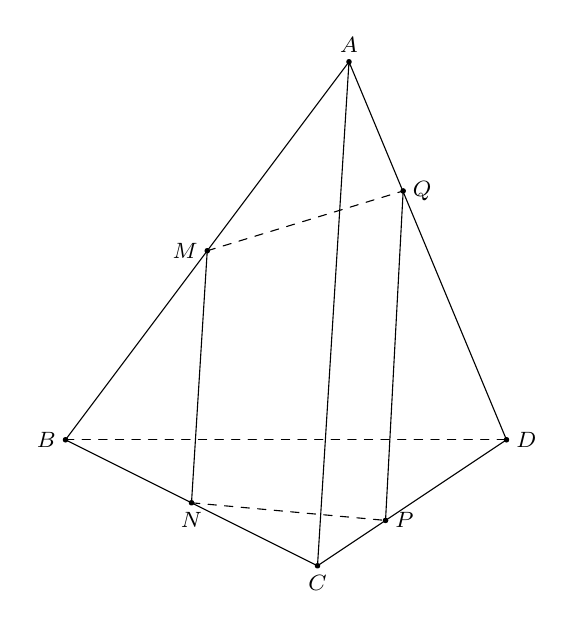
\begin{tikzpicture}[scale=0.8,font=\footnotesize, line join=round, line cap=round, >=stealth]
					\coordinate (B) at (-4,0);\draw[fill=black] (B) circle(1pt);
					\coordinate (D) at (3,0);\draw[fill=black] (D) circle(1pt);
					\coordinate (C) at (0,-2);\draw[fill=black] (C) circle(1pt);
					\coordinate (A) at (0.5,6);\draw[fill=black] (A) circle(1pt);
					\coordinate (M) at (-1.75,3);\draw[fill=black] (M) circle(1pt);
					\coordinate (N) at (-2,-1);\draw[fill=black] (N) circle(1pt);
					\coordinate (P) at (1.08,-1.28);\draw[fill=black] (P) circle(1pt);
					\coordinate (Q) at (1.36,3.95);\draw[fill=black] (Q) circle(1pt);
					\draw (B) node[left]{$B$}--(C)node[below]{$C$}--(D)node[right]{$D$}--(A)node[above]{$A$}--(C);
					\draw (B)--(A);
					\draw[dashed] (B)--(D);
					\draw (M)node[left]{$M$}--(N)node[below]{$N$};
					\draw[dashed] (N)--(P)node[right]{$P$};
					\draw[dashed] (M)--(Q)node[right]{$Q$};
					\draw (P)--(Q);
			\end{tikzpicture}}
		$\heva{&AC\parallel MN\\&AC\subset \left( ACD\right) \\&MN\subset\left( MNP\right) \\& P \in \left( ACD\right) \cap \left( MNP\right) }\Rightarrow \left( ACD\right) \cap\left( MNP\right) =Px\parallel AC\parallel MN$.\\
		Gọi $Q=Px \cap AD\Rightarrow Q=AD\cap \left( MNP\right) $.\\
Trong tam giác $ACD$ có $PQ\parallel AC$. Nên $\dfrac{AQ}{AD}=\dfrac{CP}{CD}=\dfrac{1}{3}$.
	
	}
\end{ex}
\begin{ex}%[1D5V2-3]
	Một người thống kê lại thời gian thực hiện các cuộc gọi điện thoại của người đó trong một tuần ở bảng sau:
	\begin{center}
		\begin{tabular}{|c|c|c|c|c|c|c|}
			\hline
			Thời gian (giây)& $ [0;\,60) $ & $ [60;\,120) $ & $ [120;\,180) $ & $ [180;\,240) $ & $ [240;\,300) $ & $ [300;\,360) $ \\
			\hline
			Số cuộc gọi & $ 8 $ & $ 10 $ & $ 7 $ & $ 5 $ & $ 2 $ & $ 1 $ \\
			\hline
		\end{tabular}
	\end{center}
Tứ phân vị thứ 3 của mẫu số liệu bằng
\shortans[0]{$180$}	
	\loigiai{
		Gọi $ x_1,\,\ldots\,, x_{33} $ là thời gian thực hiện các cuộc gọi trong một tuần theo thứ tự không giảm.\\
		Tứ phân vị thứ ba của mẫu số liệu là $ \dfrac{1}{2}(x_{25}+x_{26}) $ nên $ Q_3=180 $.
	}
\end{ex}
\Closesolutionfile{ans}
\indapan{6}{ans/ans-1-OTHK1-De3-KQ}

